\documentclass[a4paper,12pt]{article}
\usepackage{amsmath, amssymb, graphicx}
\usepackage[french]{babel}
\usepackage{geometry}
\geometry{margin=1in}

\begin{document}

\begin{center}
    \large
\textbf{ECO432 - mercredi 05 mars 2025 de 9h à 11h.}

\emph{Documents autorisés: dictionnaire papier et feuille A4 annotée}
\end{center}


\subsection*{Exercice 1: Questions de cours (2 points)}

Donner, sans justification, la seule bonne réponse aux questions 1 et 2. 

\begin{enumerate}
\item \textbf{[1 pt]} Quelle affirmation suivante est correcte ?
    \begin{enumerate}
        \item En pratique, les banques commerciales créent autant d'argent qu'elles le peuvent jusqu'à être limitées par le ratio de réserves obligatoires
        \item Le principal taux fixé par la banque centrale est le taux d'intérêt sur les obligations sans risque à un an
        \item La banque centrale a le monopole de la création monétaire
        \item La banque centrale peut influencer le taux d'intérêt sans risque à un an en modifiant les anticipations des agents économiques
    \end{enumerate}
\item \textbf{[1 pt]} Laquelle des affirmations suivantes est certainement vraie ?
\begin{enumerate}
    \item Lorsque plus d'agents sont contraints par le crédit, les dépenses publiques sont plus efficaces pour stimuler la demande
    \item Une demande ricardienne typique peut être représentée par $c(Y) = c_0 + c_1 Y$ où $c_1$ est la propension marginale à consommer
    \item Dans une économie avec principalement des ménages ricardiens, la demande d'investissement à court terme est plus élevée
    \item Les ménages ricardiens sont plus rationnels que les ménages keynésiens
\end{enumerate}

\end{enumerate}


\subsection*{Exercice 2: Pourquoi les riches épargnent-ils tant? (8 points)}

On considère le problème d'un agent représentatif vivant $T+1$ périodes. A chaque date $t=0,\cdots,T$ il
reçoit le revenu exogène $Y_t$ et consomme un montant $C_t$.
Pour toutes les périodes $t<T$ il peut aussi placer un montant $A_t$ rémunéré au 
taux réel $1+r$ au début de la période $t+1$. Il n'y a pas de contrainte d'endettement mais on suppose $A_T=0$.

L'agent maximise l'utilité intertemporelle: 

\begin{equation}
\sum_{t=0}^{T-1} \beta^t \left( \log(C_t) + \varphi \log(A_t) \right) + \beta^T \log(C_T)\label{objectif}
\end{equation}

où $\beta>0$ est le time discount, et où $\phi\geq0$ paramétrise la préférence pour la richesse.


On définit deux types de chocs de revenu qui peuvent arriver en période $t$ :

\begin{itemize}
\item Un choc de revenu temporaire $\Delta \xi$ qui affecte uniquement $Y_0$
\item Un choc de revenu permanent $\Delta \psi$ qui augmente le revenu à toutes les dates supérieures à $t$.
\end{itemize}

On vise ici à étudier comment la préférence pour la richesse affecte la propension marginale à consommer face à ces deux types de chocs.


\newpage

\subsubsection*{Questions}

\emph{Pour répondre aux questions 2.a et 3.a, on pourra, sans préjudice supposer $T=1$.}

\begin{enumerate}
    \item Écrire la contrainte de budget pour chaque période $t$. En supposant qu'elle est saturée montrer qu'on a la contrainte de budget intertemporelle: \hfill\textbf{[0.5 pt]} 
    \begin{equation}
    \sum_{t=0}^{T-1} \frac{C_t}{(1+r)^t} = \sum_{t=0}^{T-1} \frac{Y_t}{(1+r)^t} \label{contrainte}
    \end{equation}
    \item  On se place tout d'abord dans le cas $\varphi=0$ et on suppose $\beta (1+r)=1$.
        \begin{enumerate}
            \item Montrer que la consommation optimale est constante en maximisant l'utilité intertemporelle (\ref{objectif}) sous la contrainte de budget intertemporelle (\ref{contrainte}). \hfill \textbf{[1.5 pt]}  
            \item Quelle est la propension marginale à consommer pour un choc temporaire? Pour un choc permanent? \hfill \textbf{[1 pt]}  
            \item Comment appelle-t-on ce type d'agent? \hfill \textbf{[0.5 pt]}
        \end{enumerate} 
    
    \item On suppose désormais  $\varphi>0$.
            \begin{enumerate}
                \item Montrer que pour $t<T$ la consommation optimale satisfait: \hfill\textbf{[1.5 pt]}
                    \begin{equation}
                    \frac{C_{t+1}}{C_t} = \frac{\beta}{1+r} \left(1 + \varphi \frac{A_t}{C_t} \right)
                    \label{foc}
                    \end{equation}
                \item En supposant $T>>1$ \footnote{On ne demande pas ici une preuve de convergence. 
                On considere simplement que l'équation \ref{foc} est satisfaite à toutes les dates $t>0$ en ignorant la condition terminale.}, déterminer la valeur stationnaire de la consommation et de la richesse en fonction de $r$,$\beta$ et $\varphi$. \hfill\textbf{[1 pt]}
                \item Dans cet état stationaire, quelle est la propension marginale à consommer de l'agent lorsqu'il reçoit un choc de revenu permanent? \hfill\textbf{[1 pt]}
            \end{enumerate} 

    \item Dans les données US 
    \footnote{Source: \underline{Do the Rich Save More?} par Dynan, Skinner \& Zeldes, JPE, 2004. } 
    la propension marginale à consommer pour un choc de revenu permanent à été évaluée autour de 95\% pour les 10\% des ménages les plus pauvres et autour de $70\%$ pour les $10\%$ des ménages les plus riches. \\
    Commenter.\hfill\textbf{[1 pt]}
    \end{enumerate}


\subsection*{Exercice 3 : Modèle de Solow avec progrès technique spécifique à l’investissement (4 points)}

Le temps est continu, $t \in [0, +\infty[$. Soit une économie fermée, produisant un bien de consommation selon la fonction de production :

\begin{equation}
    Y_t = K_t^{\alpha} L_t^{1-\alpha},
\end{equation}

où $K_t$ est le stock de capital à la date $t$, $\alpha$ un paramètre compris strictement entre 0 et 1 et $L_t$ est la quantité de travail, supposée croissante au taux exogène $n > 0$ :
$\forall t\geq 0, \frac{\dot{L_t}}{L_t} = n$.

Les agents de l’économie ont un taux d’épargne constant  $s \in ]0,1]$.

Contrairement au modèle de Solow ordinaire, nous supposons ici l’existence 
de \underline{deux} biens distincts : le bien de consommation et le bien capital. 
Le bien capital est produit à partir du bien de consommation, par une technologie linéaire
et en situation de concurrence pure et parfaite. Chaque unité de bien de consommation peut
être soit consommée, soit transformée en $q_t > 0$ unités de bien capital.

Ainsi, l’équation d’accumulation du capital est :

\begin{equation}
    \dot{K_t} = - \delta K_t + s q_t Y_t,
\end{equation}

où $\delta > 0$ est le taux de dépréciation du capital, et où $q_t$ est le terme dit de "productivité
spécifique à l'investissement" et qui augmente exponentiellement : $q_t = q_0 e^{g_q t}$ avec $q_0 > 0$ et $g_q > 0$ exogènes.

A la date 0, il existe $K_0>0$ unités de capital et la population est à $L_0>0$.

\subsubsection*{Questions}

\begin{enumerate}
    \item Soit $\gamma \in \mathbb{R}$. On note $k_t = \frac{K_t}{(q_t)^\gamma L_t}$. Calculer $\frac{\dot{k_t}}{k_t}$ en fonction de $K_t, L_t, q_t$ et des paramètres. \hfill \textbf{[0.5]}
    \item Montrer que pour un certain $\gamma$ à préciser, $k_t$ obéit à une équation différentielle autonome.\footnote{C'est à dire: il existe une fonction $\phi$ telle que $\forall t, \dot{k}_t = \phi(k_t)$} \hfill \textbf{[1]}  
    \item Montrer que pour la valeur de $\gamma$ trouvée à la question précédente, $k_t$ converge vers un certain $k^* > 0$ (à préciser) lorsque $t \to \infty$. \hfill \textbf{[1.5]}
    \item Montrer que $\frac{\dot{K_t}}{K_t}$ tend vers une limite $g_K$ (à préciser) et que $\frac{\dot{Y_t}}{Y_t}$ tend vers une limite $g_Y$ (à préciser). \hfill \textbf{[1]}  
    \item Ce modèle est-il compatible avec le quatrième fait stylisé de Kaldor selon lequel le ratio capital/PIB n’a pas de tendance de long-terme ? (\emph{\underline{indication}: quel est le prix du bien capital en termes du bien de consommation ?}) \hfill \textbf{[1]}  
\end{enumerate}

\subsection*{Exercice 2 : Démographie et automatisation (6 points)}

\emph{D’après Abeliansky \& Prettner (2021) "Population growth and automation density: Theory and cross-country evidence", working paper.}

\hfill

On considère un modèle de croissance avec trois inputs : le travail $L_t$, le capital traditionnel $K_t$ et le capital d’automatisation $P_t$. La fonction de production est :

\begin{equation}
    Y_t = F(K_t, P_t, L_t) = K_t^{\alpha} (P_t + L_t)^{1-\alpha}, \quad \alpha \in ]0,1[.
\end{equation}

Les équations suivantes régissent le modèle:

\begin{align}
    K_{t+1} + P_{t+1} &= s Y_t, \\
    L_{t+1} &= (1 + n)L_t, \\
    \frac{\partial F}{\partial K_{t+1}} (K_{t+1}, P_{t+1}, L_{t+1}) &= \frac{\partial F}{\partial P_{t+1}} (K_{t+1}, P_{t+1}, L_{t+1}).
\end{align}

où $n>0$ et $s\in ]0,1]$ sont des paramètres. Les valeurs de $K_0$, $P_0$ et $L_0$ sont données et strictement positives. On suppose que $s\frac{\alpha^\alpha(1-\alpha)^{1-\alpha}}{1+n}>\alpha$.
\subsubsection*{Questions}

\begin{figure}
    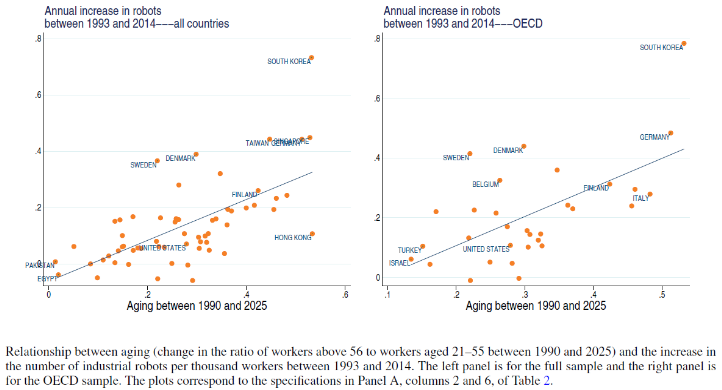
\includegraphics[width=\textwidth]{graph1.png}
    \caption{Source: Acemoglu \& Restrepo (2022). \emph{Demographics and automation (Review of Economic Studies)}}
    \label{acemoglu}
\end{figure}

\begin{enumerate}
    \item Commenter la fonction de production. \hfill  \textbf{[0.5]}
    \item Identifier les hypothèses sous-jacentes aux équations (7) et (9) du modèle. \hfill  \textbf{[1.5]}
    \item Montrer que pour tout $t \geq 0$ : \hfill  \textbf{[0.5]}
    \begin{equation}
        \frac{K_{t+1}}{P_{t+1} + L_{t+1}} = \frac{\alpha}{1-\alpha}.
    \end{equation}
    
    \item  Soit $p_t = P_t / L_t$. Trouver une relation entre $p_t$ et $p_{t+1}$,
    représenter graphiquement cette relation et montrer que $p_t$ converge vers un certain $p^*$ (à préciser).  \hfill \textbf{[1.5]}
    \item  À l’aide du modèle, comment expliquez-vous la corrélation positive en coupe entre vieillissement de la population et investissement en robots industriels représentée sur la figure \ref{acemoglu} ? \hfill \textbf{[2]}  
\end{enumerate}

\end{document}
